% Options for packages loaded elsewhere
\PassOptionsToPackage{unicode}{hyperref}
\PassOptionsToPackage{hyphens}{url}
%
\documentclass[
]{article}
\usepackage{amsmath,amssymb}
\usepackage{lmodern}
\usepackage{ifxetex,ifluatex}
\ifnum 0\ifxetex 1\fi\ifluatex 1\fi=0 % if pdftex
  \usepackage[T1]{fontenc}
  \usepackage[utf8]{inputenc}
  \usepackage{textcomp} % provide euro and other symbols
\else % if luatex or xetex
  \usepackage{unicode-math}
  \defaultfontfeatures{Scale=MatchLowercase}
  \defaultfontfeatures[\rmfamily]{Ligatures=TeX,Scale=1}
\fi
% Use upquote if available, for straight quotes in verbatim environments
\IfFileExists{upquote.sty}{\usepackage{upquote}}{}
\IfFileExists{microtype.sty}{% use microtype if available
  \usepackage[]{microtype}
  \UseMicrotypeSet[protrusion]{basicmath} % disable protrusion for tt fonts
}{}
\makeatletter
\@ifundefined{KOMAClassName}{% if non-KOMA class
  \IfFileExists{parskip.sty}{%
    \usepackage{parskip}
  }{% else
    \setlength{\parindent}{0pt}
    \setlength{\parskip}{6pt plus 2pt minus 1pt}}
}{% if KOMA class
  \KOMAoptions{parskip=half}}
\makeatother
\usepackage{xcolor}
\IfFileExists{xurl.sty}{\usepackage{xurl}}{} % add URL line breaks if available
\IfFileExists{bookmark.sty}{\usepackage{bookmark}}{\usepackage{hyperref}}
\hypersetup{
  hidelinks,
  pdfcreator={LaTeX via pandoc}}
\urlstyle{same} % disable monospaced font for URLs
\usepackage[margin=1in]{geometry}
\usepackage{color}
\usepackage{fancyvrb}
\newcommand{\VerbBar}{|}
\newcommand{\VERB}{\Verb[commandchars=\\\{\}]}
\DefineVerbatimEnvironment{Highlighting}{Verbatim}{commandchars=\\\{\}}
% Add ',fontsize=\small' for more characters per line
\usepackage{framed}
\definecolor{shadecolor}{RGB}{248,248,248}
\newenvironment{Shaded}{\begin{snugshade}}{\end{snugshade}}
\newcommand{\AlertTok}[1]{\textcolor[rgb]{0.94,0.16,0.16}{#1}}
\newcommand{\AnnotationTok}[1]{\textcolor[rgb]{0.56,0.35,0.01}{\textbf{\textit{#1}}}}
\newcommand{\AttributeTok}[1]{\textcolor[rgb]{0.77,0.63,0.00}{#1}}
\newcommand{\BaseNTok}[1]{\textcolor[rgb]{0.00,0.00,0.81}{#1}}
\newcommand{\BuiltInTok}[1]{#1}
\newcommand{\CharTok}[1]{\textcolor[rgb]{0.31,0.60,0.02}{#1}}
\newcommand{\CommentTok}[1]{\textcolor[rgb]{0.56,0.35,0.01}{\textit{#1}}}
\newcommand{\CommentVarTok}[1]{\textcolor[rgb]{0.56,0.35,0.01}{\textbf{\textit{#1}}}}
\newcommand{\ConstantTok}[1]{\textcolor[rgb]{0.00,0.00,0.00}{#1}}
\newcommand{\ControlFlowTok}[1]{\textcolor[rgb]{0.13,0.29,0.53}{\textbf{#1}}}
\newcommand{\DataTypeTok}[1]{\textcolor[rgb]{0.13,0.29,0.53}{#1}}
\newcommand{\DecValTok}[1]{\textcolor[rgb]{0.00,0.00,0.81}{#1}}
\newcommand{\DocumentationTok}[1]{\textcolor[rgb]{0.56,0.35,0.01}{\textbf{\textit{#1}}}}
\newcommand{\ErrorTok}[1]{\textcolor[rgb]{0.64,0.00,0.00}{\textbf{#1}}}
\newcommand{\ExtensionTok}[1]{#1}
\newcommand{\FloatTok}[1]{\textcolor[rgb]{0.00,0.00,0.81}{#1}}
\newcommand{\FunctionTok}[1]{\textcolor[rgb]{0.00,0.00,0.00}{#1}}
\newcommand{\ImportTok}[1]{#1}
\newcommand{\InformationTok}[1]{\textcolor[rgb]{0.56,0.35,0.01}{\textbf{\textit{#1}}}}
\newcommand{\KeywordTok}[1]{\textcolor[rgb]{0.13,0.29,0.53}{\textbf{#1}}}
\newcommand{\NormalTok}[1]{#1}
\newcommand{\OperatorTok}[1]{\textcolor[rgb]{0.81,0.36,0.00}{\textbf{#1}}}
\newcommand{\OtherTok}[1]{\textcolor[rgb]{0.56,0.35,0.01}{#1}}
\newcommand{\PreprocessorTok}[1]{\textcolor[rgb]{0.56,0.35,0.01}{\textit{#1}}}
\newcommand{\RegionMarkerTok}[1]{#1}
\newcommand{\SpecialCharTok}[1]{\textcolor[rgb]{0.00,0.00,0.00}{#1}}
\newcommand{\SpecialStringTok}[1]{\textcolor[rgb]{0.31,0.60,0.02}{#1}}
\newcommand{\StringTok}[1]{\textcolor[rgb]{0.31,0.60,0.02}{#1}}
\newcommand{\VariableTok}[1]{\textcolor[rgb]{0.00,0.00,0.00}{#1}}
\newcommand{\VerbatimStringTok}[1]{\textcolor[rgb]{0.31,0.60,0.02}{#1}}
\newcommand{\WarningTok}[1]{\textcolor[rgb]{0.56,0.35,0.01}{\textbf{\textit{#1}}}}
\usepackage{graphicx}
\makeatletter
\def\maxwidth{\ifdim\Gin@nat@width>\linewidth\linewidth\else\Gin@nat@width\fi}
\def\maxheight{\ifdim\Gin@nat@height>\textheight\textheight\else\Gin@nat@height\fi}
\makeatother
% Scale images if necessary, so that they will not overflow the page
% margins by default, and it is still possible to overwrite the defaults
% using explicit options in \includegraphics[width, height, ...]{}
\setkeys{Gin}{width=\maxwidth,height=\maxheight,keepaspectratio}
% Set default figure placement to htbp
\makeatletter
\def\fps@figure{htbp}
\makeatother
\setlength{\emergencystretch}{3em} % prevent overfull lines
\providecommand{\tightlist}{%
  \setlength{\itemsep}{0pt}\setlength{\parskip}{0pt}}
\setcounter{secnumdepth}{-\maxdimen} % remove section numbering
\usepackage{booktabs}
\usepackage{longtable}
\usepackage{array}
\usepackage{multirow}
\usepackage{wrapfig}
\usepackage{float}
\usepackage{colortbl}
\usepackage{pdflscape}
\usepackage{tabu}
\usepackage{threeparttable}
\usepackage{threeparttablex}
\usepackage[normalem]{ulem}
\usepackage{makecell}
\usepackage{xcolor}
\ifluatex
  \usepackage{selnolig}  % disable illegal ligatures
\fi

\author{}
\date{\vspace{-2.5em}}

\begin{document}

\ifdefined\ifprincipal
\else
\setlength{\parindent}{1em}
\pagestyle{fancy}
\setcounter{tocdepth}{4}
\tableofcontents

\fi

\ifdefined\ifdoblecara
\fancyhead{}{}
\fancyhead[LE,RO]{\scriptsize\rightmark}
\fancyfoot[LO,RE]{\scriptsize\slshape \leftmark}
\fancyfoot[C]{}
\fancyfoot[LE,RO]{\footnotesize\thepage}
\else
\fancyhead{}{}
\fancyhead[RO]{\scriptsize\rightmark}
\fancyfoot[LO]{\scriptsize\slshape \leftmark}
\fancyfoot[C]{}
\fancyfoot[RO]{\footnotesize\thepage}
\fi
\renewcommand{\headrulewidth}{0.4pt}
\renewcommand{\footrulewidth}{0.4pt}

Nota: Para la replicación de los resultados, haremos uso de la función
\emph{trainControl}, donde emplearemos validación cruzada con 5 grupos y
tres repeticiones. No utilizamos 10 grupos en la validación como es lo
usual debido al pequeño número de registros que tenemos.

\begin{Shaded}
\begin{Highlighting}[]
\CommentTok{\# Para todos los modelos}
\NormalTok{fitControl }\OtherTok{\textless{}{-}} \FunctionTok{trainControl}\NormalTok{(}\AttributeTok{method =} \StringTok{"repeatedcv"}\NormalTok{,}
                           \AttributeTok{number =} \DecValTok{5}\NormalTok{, }\AttributeTok{repeats =} \DecValTok{3}\NormalTok{,}
                           \AttributeTok{verboseIter =}\ConstantTok{FALSE}\NormalTok{ )}
\end{Highlighting}
\end{Shaded}

De cara a utilizar optimizar el rendimiento de los algoritmos de
regresión, haremos uso de la instrucción \emph{preProcess} de la función
\emph{train} para escalar nuestras variables y que estén todas en la
misma escala, con el objetivo de obtener mejores métricas y que los
modelo minimicen el error al predecir las ventas.

Al hacer la división de los datos para entrenar los modelos, se ha
optado por no utilizar un conjunto de datos de validación ya que
únicamente tenemos 181 registros y tener datos para validad los modelos
supondría tener aún menos registros para entrenarlos, y por tanto, se
obtendrían métricas menos precisas.

\hypertarget{divisiuxf3n-de-los-datos-en-entrenamiento-y-testeo}{%
\subparagraph{División de los datos en entrenamiento y
testeo}\label{divisiuxf3n-de-los-datos-en-entrenamiento-y-testeo}}

De cara a entrenar los modelos, se tomará una partición de 80\% y 20\%
para los datos de entrenamiento y testeo, respectivamente. De esta
manera, tomamos los 145 primeros registros para entrenar el modelo y 36
para el testeo. Esto corresponde a entrenar los modelos con datos
diarios desde el 1 de Agosto al 23 de Diciembre, para posteriormente
realizar predicciones del 24 de Diciembre al 30 de Enero.

\hypertarget{predicciuxf3n-del-volumen-total-de-ventas}{%
\subparagraph{Predicción del volumen total de
ventas}\label{predicciuxf3n-del-volumen-total-de-ventas}}

\textbf{División de los datos en entrenamiento y testeo}

Se toma una partición de 80\% 20\% para los datos de entrenamiento y
testeo:

\begin{Shaded}
\begin{Highlighting}[]
\CommentTok{\# Datos de entrenamiento}
\NormalTok{DatosEntreamiento\_Total }\OtherTok{\textless{}{-}}\NormalTok{ VolumenVentas\_TOTAL[indient,]}
\CommentTok{\# Datos de testeo}
\NormalTok{DatosTesteo\_Total}\OtherTok{\textless{}{-}}\NormalTok{VolumenVentas\_TOTAL[inditest,]}
\end{Highlighting}
\end{Shaded}

Algoritmo 1: Máquina de vector soporte (SVM)

\textbf{Hiperparámetros del algoritmo}

\begin{itemize}
\tightlist
\item
  Validación cruzada con 5 grupos y tres repeticiones
\item
  Parámetro de costo, C: malla de valores entre 1 y 3. Este parámetro
  penaliza al modelo por cometer errores. Cuanto mayor sea su valor,
  menos probable es que el algoritmo realice una predicción errónea.
\end{itemize}

\textbf{Modelado}

\begin{Shaded}
\begin{Highlighting}[]
\CommentTok{\# Malla para hiperparámetros}
\NormalTok{SVMGrid }\OtherTok{\textless{}{-}}  \FunctionTok{expand.grid}\NormalTok{(}\AttributeTok{C =} \FunctionTok{seq}\NormalTok{(}\DecValTok{1}\NormalTok{,}\DecValTok{3}\NormalTok{, }\AttributeTok{length =} \DecValTok{20}\NormalTok{))}

\FunctionTok{set.seed}\NormalTok{(}\DecValTok{17}\NormalTok{)}
\NormalTok{modeloSVM\_T }\OtherTok{\textless{}{-}} \FunctionTok{train}\NormalTok{(VENTAS}\SpecialCharTok{\textasciitilde{}}\NormalTok{., }
                \AttributeTok{data =}\NormalTok{ DatosEntreamiento\_Total[,}\SpecialCharTok{{-}}\FunctionTok{c}\NormalTok{(}\DecValTok{1}\NormalTok{,}\DecValTok{5}\NormalTok{,}\DecValTok{6}\NormalTok{)], }
                \AttributeTok{method =} \StringTok{"svmLinear"}\NormalTok{, }
                \AttributeTok{trControl=}\NormalTok{fitControl, }
                \AttributeTok{preProcess=}\FunctionTok{c}\NormalTok{(}\StringTok{"center"}\NormalTok{,}\StringTok{"scale"}\NormalTok{),}
                \AttributeTok{tuneGrid =}\NormalTok{ SVMGrid)}
\end{Highlighting}
\end{Shaded}

\textbf{Resultados}

El modelo tiene un costo \emph{C} = 1.3157895 y nos ofrece las
siguientes métricas:

\begin{table}[H]

\caption{\label{tab:unnamed-chunk-10}Métricas del mejor modelo}
\centering
\begin{tabular}[t]{lrrrrrrr}
\toprule
  & C & RMSE & Rsquared & MAE & RMSESD & RsquaredSD & MAESD\\
\midrule
4 & 1.315789 & 660.7109 & 0.6006251 & 333.5372 & 431.7381 & 0.29241 & 144.3136\\
\bottomrule
\end{tabular}
\end{table}

\textbf{Métricas del remuestreo:}

\begin{longtable}[t]{rrrl}
\caption{\label{tab:unnamed-chunk-11}Métricas en el remuestreo}\\
\toprule
RMSE & Rsquared & MAE & Resample\\
\midrule
\endfirsthead
\caption[]{Métricas en el remuestreo \textit{(continued)}}\\
\toprule
RMSE & Rsquared & MAE & Resample\\
\midrule
\endhead

\endfoot
\bottomrule
\endlastfoot
\cellcolor{gray!6}{1064.4454} & \cellcolor{gray!6}{0.3088627} & \cellcolor{gray!6}{453.5632} & \cellcolor{gray!6}{Fold2.Rep1}\\
1184.6328 & 0.2829904 & 458.7337 & Fold1.Rep1\\
\cellcolor{gray!6}{293.4512} & \cellcolor{gray!6}{0.8920958} & \cellcolor{gray!6}{223.3695} & \cellcolor{gray!6}{Fold5.Rep2}\\
1137.7534 & 0.3301661 & 394.2148 & Fold2.Rep3\\
\cellcolor{gray!6}{450.3332} & \cellcolor{gray!6}{0.7131619} & \cellcolor{gray!6}{278.7487} & \cellcolor{gray!6}{Fold4.Rep3}\\
\addlinespace
294.5183 & 0.8869078 & 209.1698 & Fold3.Rep1\\
\cellcolor{gray!6}{330.2677} & \cellcolor{gray!6}{0.8611998} & \cellcolor{gray!6}{241.7020} & \cellcolor{gray!6}{Fold5.Rep1}\\
302.5374 & 0.8720160 & 230.8551 & Fold2.Rep2\\
\cellcolor{gray!6}{1586.7542} & \cellcolor{gray!6}{0.0591160} & \cellcolor{gray!6}{701.2347} & \cellcolor{gray!6}{Fold4.Rep2}\\
1133.8313 & 0.1815909 & 529.3938 & Fold1.Rep3\\
\addlinespace
\cellcolor{gray!6}{435.7051} & \cellcolor{gray!6}{0.7702168} & \cellcolor{gray!6}{268.4395} & \cellcolor{gray!6}{Fold3.Rep3}\\
262.8688 & 0.8897975 & 200.3649 & Fold5.Rep3\\
\cellcolor{gray!6}{511.0738} & \cellcolor{gray!6}{0.5204610} & \cellcolor{gray!6}{295.4428} & \cellcolor{gray!6}{Fold4.Rep1}\\
488.7918 & 0.7056551 & 266.0491 & Fold1.Rep2\\
\cellcolor{gray!6}{433.6988} & \cellcolor{gray!6}{0.7351391} & \cellcolor{gray!6}{251.7757} & \cellcolor{gray!6}{Fold3.Rep2}\\*
\end{longtable}

Observando los resultados, llegamos lo siguiente:

\begin{itemize}
\tightlist
\item
  El modelo consigue explicar un 60.06 \% de la variabilidad total del
  volumen de ventas para los datos de entrenamiento
\item
  El error cuadrático medio es de 661 unidades
\item
  Respecto al remuestreo en la validación cruzada, vemos que las
  métricas tienen cierta variabilidad, en algunas ocasiones se obtiene
  un \(R^2\) por encima de 0.85 y en otras menor que 0.3, aunque la
  mayoría de veces se mantiene con un \(R^2\) mayor que 0.7.
\end{itemize}

En el gráfico mostrado a continuación, se puede observar la variabilidad
del error cuadrático medio en función del valor de costo:

\begin{center}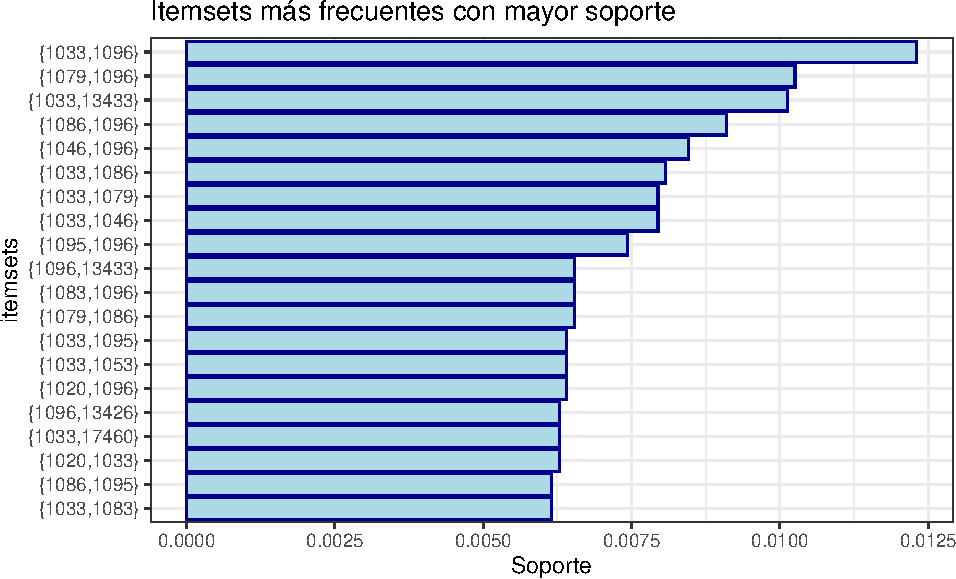
\includegraphics[width=0.95\linewidth]{figurasR/unnamed-chunk-12-1} \end{center}

A medida que el valor del costo es mayor, el RMSE aumenta
considerablemente.

Algoritmo 2: K-Nearest Neighbor Regression (KNN)

\textbf{Hiperparámetros del algoritmo}

\begin{itemize}
\tightlist
\item
  Validación cruzada con 5 grupos y tres repeticiones
\item
  Número de vecinos, k: malla para 3,5,7 y 9
\end{itemize}

\textbf{Modelado}

\begin{Shaded}
\begin{Highlighting}[]
\CommentTok{\# Malla para hiperparámetros}
\NormalTok{KNNGrid }\OtherTok{\textless{}{-}}  \FunctionTok{expand.grid}\NormalTok{(}\AttributeTok{k =} \FunctionTok{seq}\NormalTok{(}\DecValTok{3}\NormalTok{,}\DecValTok{9}\NormalTok{, }\AttributeTok{by=}\DecValTok{2}\NormalTok{))}

\FunctionTok{set.seed}\NormalTok{(}\DecValTok{17}\NormalTok{)}
\NormalTok{modeloKNN\_T }\OtherTok{\textless{}{-}} \FunctionTok{train}\NormalTok{(VENTAS}\SpecialCharTok{\textasciitilde{}}\NormalTok{., }
                \AttributeTok{data =}\NormalTok{ DatosEntreamiento\_Total[,}\SpecialCharTok{{-}}\FunctionTok{c}\NormalTok{(}\DecValTok{1}\NormalTok{,}\DecValTok{5}\NormalTok{,}\DecValTok{6}\NormalTok{)], }
                \AttributeTok{method =} \StringTok{"knn"}\NormalTok{, }
                \AttributeTok{trControl=}\NormalTok{fitControl, }
                \AttributeTok{preProcess=}\FunctionTok{c}\NormalTok{(}\StringTok{"center"}\NormalTok{,}\StringTok{"scale"}\NormalTok{),}
                \AttributeTok{tuneGrid =}\NormalTok{ KNNGrid)}
\end{Highlighting}
\end{Shaded}

\textbf{Resultados}

El con \emph{K} = 7 vecinos es el que nos proporciona mejores métricas:

\begin{table}[H]

\caption{\label{tab:unnamed-chunk-14}Métricas del mejor modelo}
\centering
\begin{tabular}[t]{lrrrrrrr}
\toprule
  & k & RMSE & Rsquared & MAE & RMSESD & RsquaredSD & MAESD\\
\midrule
3 & 7 & 692.3719 & 0.5669368 & 371.4261 & 366.764 & 0.2216798 & 128.5426\\
\bottomrule
\end{tabular}
\end{table}

\textbf{Métricas del remuestreo}

\begin{longtable}[t]{rrrl}
\caption{\label{tab:unnamed-chunk-15}Métricas en el remuestreo}\\
\toprule
RMSE & Rsquared & MAE & Resample\\
\midrule
\endfirsthead
\caption[]{Métricas en el remuestreo \textit{(continued)}}\\
\toprule
RMSE & Rsquared & MAE & Resample\\
\midrule
\endhead

\endfoot
\bottomrule
\endlastfoot
\cellcolor{gray!6}{1104.5804} & \cellcolor{gray!6}{0.3741021} & \cellcolor{gray!6}{496.7094} & \cellcolor{gray!6}{Fold1.Rep1}\\
949.8946 & 0.4590495 & 439.4187 & Fold2.Rep1\\
\cellcolor{gray!6}{1572.4870} & \cellcolor{gray!6}{0.0765971} & \cellcolor{gray!6}{705.3367} & \cellcolor{gray!6}{Fold4.Rep2}\\
523.3315 & 0.6660395 & 322.7905 & Fold1.Rep2\\
\cellcolor{gray!6}{517.1772} & \cellcolor{gray!6}{0.6404919} & \cellcolor{gray!6}{294.8424} & \cellcolor{gray!6}{Fold3.Rep1}\\
\addlinespace
504.1204 & 0.6978479 & 306.0102 & Fold3.Rep3\\
\cellcolor{gray!6}{323.0070} & \cellcolor{gray!6}{0.8668280} & \cellcolor{gray!6}{244.0887} & \cellcolor{gray!6}{Fold5.Rep2}\\
330.3074 & 0.8507064 & 238.5459 & Fold2.Rep2\\
\cellcolor{gray!6}{501.5117} & \cellcolor{gray!6}{0.5115971} & \cellcolor{gray!6}{305.9048} & \cellcolor{gray!6}{Fold4.Rep1}\\
463.9028 & 0.6934043 & 292.8079 & Fold4.Rep3\\
\addlinespace
\cellcolor{gray!6}{1025.1152} & \cellcolor{gray!6}{0.3177601} & \cellcolor{gray!6}{530.6378} & \cellcolor{gray!6}{Fold1.Rep3}\\
587.9297 & 0.5137595 & 350.6238 & Fold3.Rep2\\
\cellcolor{gray!6}{370.3185} & \cellcolor{gray!6}{0.8340566} & \cellcolor{gray!6}{268.3980} & \cellcolor{gray!6}{Fold5.Rep1}\\
514.0675 & 0.6271062 & 334.1000 & Fold5.Rep3\\
\cellcolor{gray!6}{1097.8273} & \cellcolor{gray!6}{0.3747050} & \cellcolor{gray!6}{441.1762} & \cellcolor{gray!6}{Fold2.Rep3}\\*
\end{longtable}

Observando los resultados, llegamos lo siguiente:

\begin{itemize}
\tightlist
\item
  El modelo consigue explicar un 56.69 \% de la variabilidad total del
  volumen de ventas para los datos de entrenamiento
\item
  El error cuadrático medio es de 661 unidades
\item
  Respecto al remuestreo en la validación cruzada, observamos mayor
  variación de las métricas, llegando a obtener un \(R^2\) mayor que
  0.86, pero obteniendo valores menores que 0.35 en más de una ocasión.
  La variabilidad indica que el modelo no será tan robusto y por tanto,
  que las métricas serán menos fiables.
\end{itemize}

Algoritmo 3: Extreme Gradient Boosting (XGBoost)

\textbf{Hiperparámetros del algoritmo}

\begin{itemize}
\tightlist
\item
  Validación cruzada con 5 grupos y tres repeticiones
\item
  Número de pruebas de hiperparametrización (tune length): 5
\end{itemize}

\textbf{Modelado}

\begin{Shaded}
\begin{Highlighting}[]
\FunctionTok{set.seed}\NormalTok{(}\DecValTok{17}\NormalTok{)}
\NormalTok{modeloXGB\_T }\OtherTok{\textless{}{-}} \FunctionTok{train}\NormalTok{(VENTAS}\SpecialCharTok{\textasciitilde{}}\NormalTok{., }
                \AttributeTok{data =}\NormalTok{ DatosEntreamiento\_Total[,}\SpecialCharTok{{-}}\FunctionTok{c}\NormalTok{(}\DecValTok{1}\NormalTok{,}\DecValTok{5}\NormalTok{,}\DecValTok{6}\NormalTok{)], }
                \AttributeTok{method =} \StringTok{"xgbTree"}\NormalTok{,}
                \AttributeTok{trControl=}\NormalTok{fitControl, }
                \AttributeTok{preProcess=}\FunctionTok{c}\NormalTok{(}\StringTok{"center"}\NormalTok{,}\StringTok{"scale"}\NormalTok{),}
                \AttributeTok{tuneLength=}\DecValTok{5}\NormalTok{, }\AttributeTok{verbosity=}\DecValTok{0}\NormalTok{)}
\end{Highlighting}
\end{Shaded}

\textbf{Resultados}

A continuación mostramos la configuración del mejor modelo y las
métricas obtenidas:

\begin{table}[H]

\caption{\label{tab:unnamed-chunk-17}Métricas del mejor modelo}
\centering
\resizebox{\linewidth}{!}{
\begin{tabular}[t]{lrrrrrrrrrrrrr}
\toprule
  & eta & max\_depth & gamma & colsample\_bytree & min\_child\_weight & subsample & nrounds & RMSE & Rsquared & MAE & RMSESD & RsquaredSD & MAESD\\
\midrule
\cellcolor{gray!6}{131} & \cellcolor{gray!6}{0.3} & \cellcolor{gray!6}{3} & \cellcolor{gray!6}{0} & \cellcolor{gray!6}{0.8} & \cellcolor{gray!6}{1} & \cellcolor{gray!6}{0.625} & \cellcolor{gray!6}{50} & \cellcolor{gray!6}{743.499} & \cellcolor{gray!6}{0.5273148} & \cellcolor{gray!6}{436.3185} & \cellcolor{gray!6}{353.9052} & \cellcolor{gray!6}{0.2188667} & \cellcolor{gray!6}{129.5907}\\
\bottomrule
\end{tabular}}
\end{table}

\textbf{Métricas del remuestreo:}

\begin{longtable}[t]{rrrl}
\caption{\label{tab:unnamed-chunk-18}Métricas en el remuestreo}\\
\toprule
RMSE & Rsquared & MAE & Resample\\
\midrule
\endfirsthead
\caption[]{Métricas en el remuestreo \textit{(continued)}}\\
\toprule
RMSE & Rsquared & MAE & Resample\\
\midrule
\endhead

\endfoot
\bottomrule
\endlastfoot
\cellcolor{gray!6}{658.1651} & \cellcolor{gray!6}{0.4534891} & \cellcolor{gray!6}{453.1551} & \cellcolor{gray!6}{Fold3.Rep2}\\
310.0093 & 0.8663871 & 234.6697 & Fold2.Rep2\\
\cellcolor{gray!6}{641.9839} & \cellcolor{gray!6}{0.6267043} & \cellcolor{gray!6}{393.1929} & \cellcolor{gray!6}{Fold3.Rep3}\\
962.6520 & 0.4458194 & 436.4683 & Fold2.Rep1\\
\cellcolor{gray!6}{435.8219} & \cellcolor{gray!6}{0.7575645} & \cellcolor{gray!6}{348.1510} & \cellcolor{gray!6}{Fold5.Rep2}\\
\addlinespace
551.9624 & 0.4987414 & 391.8281 & Fold4.Rep1\\
\cellcolor{gray!6}{1070.7182} & \cellcolor{gray!6}{0.2691665} & \cellcolor{gray!6}{541.5561} & \cellcolor{gray!6}{Fold1.Rep3}\\
421.4844 & 0.7818069 & 309.6371 & Fold1.Rep2\\
\cellcolor{gray!6}{515.9163} & \cellcolor{gray!6}{0.6581036} & \cellcolor{gray!6}{407.1163} & \cellcolor{gray!6}{Fold4.Rep3}\\
1560.0187 & 0.1103231 & 726.9542 & Fold4.Rep2\\
\addlinespace
\cellcolor{gray!6}{804.5749} & \cellcolor{gray!6}{0.3864338} & \cellcolor{gray!6}{496.3289} & \cellcolor{gray!6}{Fold5.Rep3}\\
1101.5879 & 0.3596894 & 536.2408 & Fold2.Rep3\\
\cellcolor{gray!6}{1147.4879} & \cellcolor{gray!6}{0.3254675} & \cellcolor{gray!6}{614.1487} & \cellcolor{gray!6}{Fold1.Rep1}\\
557.8004 & 0.5874277 & 353.0493 & Fold3.Rep1\\
\cellcolor{gray!6}{412.3023} & \cellcolor{gray!6}{0.7825979} & \cellcolor{gray!6}{302.2813} & \cellcolor{gray!6}{Fold5.Rep1}\\*
\end{longtable}

Con estos resultados:

\begin{itemize}
\tightlist
\item
  El mejor modelo consigue explicar un 52.73 \% de la variabilidad total
  del volumen de ventas para los datos de entrenamiento
\item
  El error cuadrático medio es de 743 unidades
\item
  Respecto al remuestreo en la validación cruzada, vuelve a ocurrir como
  con el segundo modelo, existe mucha variabilidad en las métricas. En
  ocasiones el modelo predice el volumen de ventas consiguiendo explicar
  más de un 85\% de la variabilidad total y en otros casos lo hace
  bastante mal. El coeficiente de determinación varía entre un valor de
  0.1103231 y 0.8663871, por lo que las predicciones no tienen mucha
  fiabilidad.
\end{itemize}

Prueba de los modelos en los datos de testeo y elección del modelo final

Configuramos los tres modelos con los mejores hiperparámetros y
mostramos a continuación una tabla con el coeficiente de determinación y
el error cuadrático medio de los tres modelos para poder seleccionar un
modelo óptimo que aplicar a los datos de testeo:

\begin{table}[H]
\centering
\begin{tabular}{lrr}
\toprule
Modelo & RMSE & R2\\
\midrule
\cellcolor{gray!6}{SVM} & \cellcolor{gray!6}{660.7109} & \cellcolor{gray!6}{0.6006251}\\
KNN & 692.3719 & 0.5669368\\
\cellcolor{gray!6}{XGBoost} & \cellcolor{gray!6}{439.0573} & \cellcolor{gray!6}{0.5220638}\\
\bottomrule
\end{tabular}
\end{table}

Observando la tabla, el modelo seleccionado para predecir el volumen
total de ventas en los datos de testeo es el modelo de máquina de vector
soporte, ya que a pesar de no tener el mejor valor de RMSE, es el que
mayor valor del coeficiente de determinación ofrece. Además, era el
modelo más robusto, al tener menor variabilidad las métricas en el
remuestreo.

\textbf{Predicción del volumen total de ventas para el conjunto de datos
test}

\begin{longtable}[t]{lrrr}
\caption{\label{tab:unnamed-chunk-20}Máquina de vector soporte}\\
\toprule
Fecha & Predicción & Valor real & Error absoluto en la predicción\\
\midrule
\endfirsthead
\caption[]{Máquina de vector soporte \textit{(continued)}}\\
\toprule
Fecha & Predicción & Valor real & Error absoluto en la predicción\\
\midrule
\endhead

\endfoot
\bottomrule
\endlastfoot
\cellcolor{gray!6}{2020-12-24} & \cellcolor{gray!6}{2064} & \cellcolor{gray!6}{2090} & \cellcolor{gray!6}{26}\\
2020-12-26 & 2675 & 340 & 2335\\
\cellcolor{gray!6}{2020-12-27} & \cellcolor{gray!6}{217} & \cellcolor{gray!6}{348} & \cellcolor{gray!6}{131}\\
2020-12-28 & 2304 & 3004 & 700\\
\cellcolor{gray!6}{2020-12-29} & \cellcolor{gray!6}{2067} & \cellcolor{gray!6}{2770} & \cellcolor{gray!6}{703}\\
\addlinespace
2020-12-30 & 2116 & 2637 & 521\\
\cellcolor{gray!6}{2020-12-31} & \cellcolor{gray!6}{2066} & \cellcolor{gray!6}{2013} & \cellcolor{gray!6}{53}\\
2021-01-02 & 2675 & 2642 & 33\\
\cellcolor{gray!6}{2021-01-03} & \cellcolor{gray!6}{231} & \cellcolor{gray!6}{191} & \cellcolor{gray!6}{40}\\
2021-01-04 & 2304 & 2951 & 647\\
\addlinespace
\cellcolor{gray!6}{2021-01-05} & \cellcolor{gray!6}{2075} & \cellcolor{gray!6}{2898} & \cellcolor{gray!6}{823}\\
2021-01-06 & 2150 & 30 & 2120\\
\cellcolor{gray!6}{2021-01-07} & \cellcolor{gray!6}{2068} & \cellcolor{gray!6}{2599} & \cellcolor{gray!6}{531}\\
2021-01-08 & 2255 & 2884 & 629\\
\cellcolor{gray!6}{2021-01-09} & \cellcolor{gray!6}{2669} & \cellcolor{gray!6}{2546} & \cellcolor{gray!6}{123}\\
\addlinespace
2021-01-10 & 207 & 161 & 46\\
\cellcolor{gray!6}{2021-01-11} & \cellcolor{gray!6}{2307} & \cellcolor{gray!6}{2492} & \cellcolor{gray!6}{185}\\
2021-01-12 & 2064 & 2496 & 432\\
\cellcolor{gray!6}{2021-01-13} & \cellcolor{gray!6}{2127} & \cellcolor{gray!6}{2116} & \cellcolor{gray!6}{11}\\
2021-01-14 & 2072 & 2058 & 14\\
\addlinespace
\cellcolor{gray!6}{2021-01-15} & \cellcolor{gray!6}{2248} & \cellcolor{gray!6}{2607} & \cellcolor{gray!6}{359}\\
2021-01-16 & 2669 & 2859 & 190\\
\cellcolor{gray!6}{2021-01-17} & \cellcolor{gray!6}{228} & \cellcolor{gray!6}{99} & \cellcolor{gray!6}{129}\\
2021-01-18 & 2298 & 2399 & 101\\
\cellcolor{gray!6}{2021-01-19} & \cellcolor{gray!6}{2068} & \cellcolor{gray!6}{2153} & \cellcolor{gray!6}{85}\\
\addlinespace
2021-01-20 & 2117 & 1830 & 287\\
\cellcolor{gray!6}{2021-01-21} & \cellcolor{gray!6}{2066} & \cellcolor{gray!6}{2100} & \cellcolor{gray!6}{34}\\
2021-01-22 & 2257 & 2433 & 176\\
\cellcolor{gray!6}{2021-01-23} & \cellcolor{gray!6}{2665} & \cellcolor{gray!6}{2992} & \cellcolor{gray!6}{327}\\
2021-01-24 & 215 & 118 & 97\\
\addlinespace
\cellcolor{gray!6}{2021-01-25} & \cellcolor{gray!6}{2295} & \cellcolor{gray!6}{2407} & \cellcolor{gray!6}{112}\\
2021-01-26 & 2067 & 2094 & 27\\
\cellcolor{gray!6}{2021-01-27} & \cellcolor{gray!6}{2123} & \cellcolor{gray!6}{2373} & \cellcolor{gray!6}{250}\\
2021-01-28 & 2065 & 2306 & 241\\
\cellcolor{gray!6}{2021-01-29} & \cellcolor{gray!6}{2259} & \cellcolor{gray!6}{2621} & \cellcolor{gray!6}{362}\\
\addlinespace
2021-01-30 & 2673 & 2966 & 293\\*
\end{longtable}

Nota: se ha obtenido en una ocasión una predicción de ventas negativa.

\begin{verbatim}
##        RMSE    Rsquared         MAE 
## 624.0146677   0.5860334 365.9166667
\end{verbatim}

El modelo \emph{máquina de vector soporte} explica un 58.6\% de la
variabilidad total del volumen de ventas en los datos de testeo. Esta
métrica ha mejorado, indicando que el modelo ha sabido generalizar con
datos nuevos. El RMSE tiene un valor alto para el volumen de ventas
diario, ya que hay un error de unas 624 ventas.

\hypertarget{predicciuxf3n-del-volumen-de-ventas-del-producto-con-calcio}{%
\subparagraph{Predicción del volumen de ventas del producto con
calcio}\label{predicciuxf3n-del-volumen-de-ventas-del-producto-con-calcio}}

\textbf{División de los datos en entrenamiento y testeo}

Tomamos una partición de 80\% 20\% para los datos de entrenamiento y
testeo:

\begin{Shaded}
\begin{Highlighting}[]
\CommentTok{\# Datos de entrenamiento}
\NormalTok{DatosEntreamiento\_Calcio }\OtherTok{\textless{}{-}}\NormalTok{ VolumenVentas\_CALCIO[indient,]}
\CommentTok{\# Datos de testeo}
\NormalTok{DatosTesteo\_Calcio}\OtherTok{\textless{}{-}}\NormalTok{VolumenVentas\_CALCIO[inditest,]}
\end{Highlighting}
\end{Shaded}

Algoritmo 1: Máquina de vector soporte (SVM)

\textbf{Hiperparámetros del algoritmo}

\begin{itemize}
\tightlist
\item
  Validación cruzada con 5 grupos y tres repeticiones
\item
  Parámetro de costo, C: malla de valores entre 1 y 3. Este parámetro
  penaliza al modelo por cometer errores. Cuanto mayor sea su valor,
  menos probable es que el algoritmo realice una predicción errónea.
\end{itemize}

\textbf{Modelado}

\begin{Shaded}
\begin{Highlighting}[]
\CommentTok{\# Malla para hiperparámetros}
\CommentTok{\# SVMGrid \textless{}{-}  expand.grid(C = seq(1,3, length = 20))}

\FunctionTok{set.seed}\NormalTok{(}\DecValTok{17}\NormalTok{)}
\NormalTok{modeloSVM\_C }\OtherTok{\textless{}{-}} \FunctionTok{train}\NormalTok{(VENTAS}\SpecialCharTok{\textasciitilde{}}\NormalTok{., }
                \AttributeTok{data =}\NormalTok{ DatosEntreamiento\_Calcio[,}\SpecialCharTok{{-}}\FunctionTok{c}\NormalTok{(}\DecValTok{1}\NormalTok{,}\DecValTok{5}\NormalTok{,}\DecValTok{6}\NormalTok{)], }
                \AttributeTok{method =} \StringTok{"svmLinear"}\NormalTok{, }
                \AttributeTok{trControl=}\NormalTok{fitControl, }
                \AttributeTok{preProcess=}\FunctionTok{c}\NormalTok{(}\StringTok{"center"}\NormalTok{,}\StringTok{"scale"}\NormalTok{),}
                \AttributeTok{tuneGrid =}\NormalTok{ SVMGrid)}
\end{Highlighting}
\end{Shaded}

\textbf{Resultados}

El modelo con un costo \emph{C} = 2.4736842 es el que proporciona
mejores métricas:

\begin{table}[H]

\caption{\label{tab:unnamed-chunk-24}Métricas del mejor modelo}
\centering
\begin{tabular}[t]{lrrrrrrr}
\toprule
  & C & RMSE & Rsquared & MAE & RMSESD & RsquaredSD & MAESD\\
\midrule
15 & 2.473684 & 410.053 & 0.5084297 & 200.9021 & 242.3671 & 0.2861008 & 75.31495\\
\bottomrule
\end{tabular}
\end{table}

\textbf{Métricas del remuestreo:}

\begin{longtable}[t]{rrrl}
\caption{\label{tab:unnamed-chunk-25}Métricas en el remuestreo}\\
\toprule
RMSE & Rsquared & MAE & Resample\\
\midrule
\endfirsthead
\caption[]{Métricas en el remuestreo \textit{(continued)}}\\
\toprule
RMSE & Rsquared & MAE & Resample\\
\midrule
\endhead

\endfoot
\bottomrule
\endlastfoot
\cellcolor{gray!6}{605.2194} & \cellcolor{gray!6}{0.1393749} & \cellcolor{gray!6}{273.8335} & \cellcolor{gray!6}{Fold2.Rep1}\\
262.0413 & 0.7387940 & 157.8381 & Fold1.Rep1\\
\cellcolor{gray!6}{251.6186} & \cellcolor{gray!6}{0.7383878} & \cellcolor{gray!6}{151.9177} & \cellcolor{gray!6}{Fold4.Rep3}\\
695.3437 & 0.2637021 & 246.0499 & Fold3.Rep1\\
\cellcolor{gray!6}{224.5364} & \cellcolor{gray!6}{0.7784103} & \cellcolor{gray!6}{134.4654} & \cellcolor{gray!6}{Fold5.Rep1}\\
\addlinespace
747.3853 & 0.0781575 & 317.9821 & Fold2.Rep2\\
\cellcolor{gray!6}{741.8805} & \cellcolor{gray!6}{0.1906661} & \cellcolor{gray!6}{282.7726} & \cellcolor{gray!6}{Fold4.Rep2}\\
316.2545 & 0.3271437 & 174.8301 & Fold1.Rep3\\
\cellcolor{gray!6}{237.5538} & \cellcolor{gray!6}{0.7685589} & \cellcolor{gray!6}{145.4539} & \cellcolor{gray!6}{Fold3.Rep3}\\
225.7057 & 0.7597007 & 149.7741 & Fold5.Rep3\\
\addlinespace
\cellcolor{gray!6}{273.5356} & \cellcolor{gray!6}{0.5252290} & \cellcolor{gray!6}{169.9023} & \cellcolor{gray!6}{Fold4.Rep1}\\
238.7011 & 0.6690615 & 171.9758 & Fold1.Rep2\\
\cellcolor{gray!6}{209.9762} & \cellcolor{gray!6}{0.8234289} & \cellcolor{gray!6}{116.4137} & \cellcolor{gray!6}{Fold3.Rep2}\\
250.9025 & 0.7109831 & 158.5497 & Fold5.Rep2\\
\cellcolor{gray!6}{870.1407} & \cellcolor{gray!6}{0.1148477} & \cellcolor{gray!6}{361.7720} & \cellcolor{gray!6}{Fold2.Rep3}\\*
\end{longtable}

Observando los resultados, llegamos lo siguiente:

\begin{itemize}
\tightlist
\item
  El modelo consigue explicar un 50.84 \% de la variabilidad total del
  volumen de ventas para los datos de entrenamiento, siendo por tanto el
  mejor modelo obtenido hasta el momento
\item
  El error cuadrático medio es de 410 unidades
\item
  Respecto al remuestreo en la validación cruzada, la variabilidad es
  evidente, en ciertas ocasiones predice muy mal y en otras lo hace algo
  mejor, aunque en la mayoría de ocasiones el \(R^2\) se mantiene
  alrededor de un 77\%.
\end{itemize}

En el gráfico mostrado a continuación, se muestra la variabilidad del
error cuadrático medio en función del valor de costo:

\begin{center}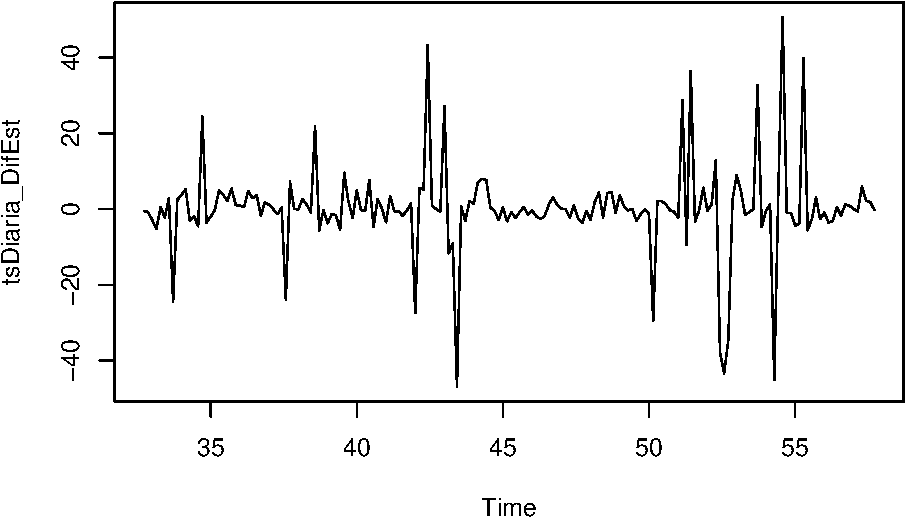
\includegraphics[width=0.95\linewidth]{figurasR/unnamed-chunk-26-1} \end{center}

Del gráfico podemos concluir que a medida que el costo es mayor, el
error cuadrático medio disminuye considerable.

Algoritmo 2: K-Nearest Neighbor Regression (KNN)

\textbf{Hiperparámetros del algoritmo}

\begin{itemize}
\tightlist
\item
  Validación cruzada con 5 grupos y tres repeticiones
\item
  Número de vecinos, k: malla para 3,5,7 y 9
\end{itemize}

\textbf{Modelado}

\begin{Shaded}
\begin{Highlighting}[]
\CommentTok{\# Malla para hiperparámetros}
\CommentTok{\# KNNGrid \textless{}{-}  expand.grid(k = seq(3,9, by=2))}

\FunctionTok{set.seed}\NormalTok{(}\DecValTok{17}\NormalTok{)}
\NormalTok{modeloKNN\_C }\OtherTok{\textless{}{-}} \FunctionTok{train}\NormalTok{(VENTAS}\SpecialCharTok{\textasciitilde{}}\NormalTok{., }
                \AttributeTok{data =}\NormalTok{ DatosEntreamiento\_Calcio[,}\SpecialCharTok{{-}}\FunctionTok{c}\NormalTok{(}\DecValTok{1}\NormalTok{,}\DecValTok{5}\NormalTok{,}\DecValTok{6}\NormalTok{)], }
                \AttributeTok{method =} \StringTok{"knn"}\NormalTok{, }
                \AttributeTok{trControl=}\NormalTok{fitControl, }
                \AttributeTok{preProcess=}\FunctionTok{c}\NormalTok{(}\StringTok{"center"}\NormalTok{,}\StringTok{"scale"}\NormalTok{),}
                \AttributeTok{tuneGrid =}\NormalTok{ KNNGrid)}
\end{Highlighting}
\end{Shaded}

\textbf{Resultados}

El modelo que nos ofrece mejores métricas utiliza 3 vecinos, \emph{K} =
9:

\begin{table}[H]

\caption{\label{tab:unnamed-chunk-28}Métricas del mejor modelo}
\centering
\begin{tabular}[t]{lrrrrrrr}
\toprule
  & k & RMSE & Rsquared & MAE & RMSESD & RsquaredSD & MAESD\\
\midrule
4 & 9 & 427.7454 & 0.4770314 & 234.2056 & 195.8891 & 0.2090557 & 65.06783\\
\bottomrule
\end{tabular}
\end{table}

\textbf{Métricas del remuestreo:}

\begin{longtable}[t]{rrrl}
\caption{\label{tab:unnamed-chunk-29}Métricas en el remuestreo}\\
\toprule
RMSE & Rsquared & MAE & Resample\\
\midrule
\endfirsthead
\caption[]{Métricas en el remuestreo \textit{(continued)}}\\
\toprule
RMSE & Rsquared & MAE & Resample\\
\midrule
\endhead

\endfoot
\bottomrule
\endlastfoot
\cellcolor{gray!6}{337.8814} & \cellcolor{gray!6}{0.6040258} & \cellcolor{gray!6}{227.8145} & \cellcolor{gray!6}{Fold1.Rep1}\\
585.0154 & 0.1880977 & 325.5011 & Fold2.Rep1\\
\cellcolor{gray!6}{888.5876} & \cellcolor{gray!6}{0.0694378} & \cellcolor{gray!6}{393.2268} & \cellcolor{gray!6}{Fold2.Rep3}\\
681.4902 & 0.3299663 & 277.9242 & Fold4.Rep2\\
\cellcolor{gray!6}{350.2643} & \cellcolor{gray!6}{0.4001104} & \cellcolor{gray!6}{245.8416} & \cellcolor{gray!6}{Fold1.Rep2}\\
\addlinespace
658.1906 & 0.3373078 & 264.7352 & Fold3.Rep1\\
\cellcolor{gray!6}{251.5721} & \cellcolor{gray!6}{0.7391376} & \cellcolor{gray!6}{163.6813} & \cellcolor{gray!6}{Fold3.Rep3}\\
261.4012 & 0.7086706 & 160.2794 & Fold5.Rep2\\
\cellcolor{gray!6}{545.5286} & \cellcolor{gray!6}{0.3263769} & \cellcolor{gray!6}{256.0068} & \cellcolor{gray!6}{Fold2.Rep2}\\
267.6461 & 0.5366879 & 171.8176 & Fold4.Rep1\\
\addlinespace
\cellcolor{gray!6}{320.6031} & \cellcolor{gray!6}{0.6221833} & \cellcolor{gray!6}{192.9137} & \cellcolor{gray!6}{Fold4.Rep3}\\
365.9266 & 0.3394912 & 252.7181 & Fold1.Rep3\\
\cellcolor{gray!6}{366.9094} & \cellcolor{gray!6}{0.5378500} & \cellcolor{gray!6}{216.6215} & \cellcolor{gray!6}{Fold3.Rep2}\\
264.6844 & 0.7083285 & 179.0464 & Fold5.Rep1\\
\cellcolor{gray!6}{270.4791} & \cellcolor{gray!6}{0.7077993} & \cellcolor{gray!6}{184.9561} & \cellcolor{gray!6}{Fold5.Rep3}\\*
\end{longtable}

Observando los resultados, llegamos lo siguiente:

\begin{itemize}
\tightlist
\item
  El mejor modelo consigue explicar un 47.7 \% de la variabilidad total
  del volumen de ventas para los datos de entrenamiento
\item
  El error cuadrático medio del mejor modelo es de 410 unidades
\item
  Respecto al remuestreo en la validación cruzada, observamos que las
  métricas presentan cierta variabilidad, llegando a obtener un \(R^2\)
  alrededor de 0.739 en alguna ocasión, aunque también se obtienen
  valores menores que 0.1 varias veces.
\end{itemize}

Algoritmo 3: Extreme Gradient Boosting (XGBoost)

\textbf{Hiperparámetros del algoritmo}

\begin{itemize}
\tightlist
\item
  Validación cruzada con 5 grupos y tres repeticiones
\item
  Número de pruebas de hiperparametrización (tune length): 5
\end{itemize}

\textbf{Modelado}

\begin{Shaded}
\begin{Highlighting}[]
\FunctionTok{set.seed}\NormalTok{(}\DecValTok{17}\NormalTok{)}
\NormalTok{modeloXGB\_C }\OtherTok{\textless{}{-}} \FunctionTok{train}\NormalTok{(VENTAS}\SpecialCharTok{\textasciitilde{}}\NormalTok{., }
                \AttributeTok{data =}\NormalTok{ DatosEntreamiento\_Calcio[,}\SpecialCharTok{{-}}\FunctionTok{c}\NormalTok{(}\DecValTok{1}\NormalTok{,}\DecValTok{5}\NormalTok{,}\DecValTok{6}\NormalTok{)], }
                \AttributeTok{method =} \StringTok{"xgbTree"}\NormalTok{,}
                \AttributeTok{trControl=}\NormalTok{fitControl, }
                \AttributeTok{preProcess=}\FunctionTok{c}\NormalTok{(}\StringTok{"center"}\NormalTok{,}\StringTok{"scale"}\NormalTok{),}
                \AttributeTok{tuneLength=}\DecValTok{5}\NormalTok{,}
                \AttributeTok{verbosity=}\DecValTok{0}\NormalTok{)}
\end{Highlighting}
\end{Shaded}

\textbf{Resultados}

A continuación mostramos la configuración del mejor modelo y las
métricas obtenidas:

\begin{table}[H]

\caption{\label{tab:unnamed-chunk-31}Métricas del mejor modelo}
\centering
\resizebox{\linewidth}{!}{
\begin{tabular}[t]{lrrrrrrrrrrrrr}
\toprule
  & eta & max\_depth & gamma & colsample\_bytree & min\_child\_weight & subsample & nrounds & RMSE & Rsquared & MAE & RMSESD & RsquaredSD & MAESD\\
\midrule
\cellcolor{gray!6}{269} & \cellcolor{gray!6}{0.4} & \cellcolor{gray!6}{1} & \cellcolor{gray!6}{0} & \cellcolor{gray!6}{0.6} & \cellcolor{gray!6}{1} & \cellcolor{gray!6}{0.875} & \cellcolor{gray!6}{200} & \cellcolor{gray!6}{417.2405} & \cellcolor{gray!6}{0.4994309} & \cellcolor{gray!6}{254.2198} & \cellcolor{gray!6}{204.0493} & \cellcolor{gray!6}{0.2414415} & \cellcolor{gray!6}{63.16719}\\
\bottomrule
\end{tabular}}
\end{table}

\textbf{Métricas del remuestreo:}

\begin{longtable}[t]{rrrl}
\caption{\label{tab:unnamed-chunk-32}Métricas en el remuestreo}\\
\toprule
RMSE & Rsquared & MAE & Resample\\
\midrule
\endfirsthead
\caption[]{Métricas en el remuestreo \textit{(continued)}}\\
\toprule
RMSE & Rsquared & MAE & Resample\\
\midrule
\endhead

\endfoot
\bottomrule
\endlastfoot
\cellcolor{gray!6}{663.2970} & \cellcolor{gray!6}{0.3396104} & \cellcolor{gray!6}{306.1226} & \cellcolor{gray!6}{Fold3.Rep1}\\
436.0698 & 0.2838283 & 328.1094 & Fold1.Rep2\\
\cellcolor{gray!6}{550.4014} & \cellcolor{gray!6}{0.3151969} & \cellcolor{gray!6}{275.3378} & \cellcolor{gray!6}{Fold2.Rep2}\\
227.2224 & 0.7572851 & 189.8796 & Fold5.Rep3\\
\cellcolor{gray!6}{572.0858} & \cellcolor{gray!6}{0.2168972} & \cellcolor{gray!6}{307.4326} & \cellcolor{gray!6}{Fold2.Rep1}\\
\addlinespace
405.4052 & 0.3107259 & 287.6732 & Fold4.Rep1\\
\cellcolor{gray!6}{690.2166} & \cellcolor{gray!6}{0.3167046} & \cellcolor{gray!6}{280.9844} & \cellcolor{gray!6}{Fold4.Rep2}\\
259.8125 & 0.7361796 & 203.2105 & Fold3.Rep2\\
\cellcolor{gray!6}{254.8398} & \cellcolor{gray!6}{0.6952834} & \cellcolor{gray!6}{189.3072} & \cellcolor{gray!6}{Fold5.Rep2}\\
225.5202 & 0.7764179 & 180.8268 & Fold5.Rep1\\
\addlinespace
\cellcolor{gray!6}{326.4058} & \cellcolor{gray!6}{0.4068394} & \cellcolor{gray!6}{252.4158} & \cellcolor{gray!6}{Fold1.Rep3}\\
218.4057 & 0.8112577 & 175.8185 & Fold3.Rep3\\
\cellcolor{gray!6}{298.8358} & \cellcolor{gray!6}{0.6614095} & \cellcolor{gray!6}{230.0529} & \cellcolor{gray!6}{Fold4.Rep3}\\
861.7966 & 0.1298035 & 388.9337 & Fold2.Rep3\\
\cellcolor{gray!6}{268.2929} & \cellcolor{gray!6}{0.7340241} & \cellcolor{gray!6}{217.1924} & \cellcolor{gray!6}{Fold1.Rep1}\\*
\end{longtable}

Observando los resultados, llegamos lo siguiente:

\begin{itemize}
\tightlist
\item
  El mejor modelo consigue explicar un 49.94 \% de la variabilidad total
  del volumen de ventas para los datos de entrenamiento
\item
  El error cuadrático medio es de 417 unidades
\item
  Respecto al remuestreo en la validación cruzada, se trata de un modelo
  donde obtenemos un valor de \(R^2\) por encima del 65\% en la mayoría
  de ocasiones. El coeficiente de determinación varía entre un valor de
  0.1298035 y 0.8112577, por lo que las predicciones serán más fiables
  que en el resto de modelos.
\end{itemize}

Prueba de los modelos en los datos de testeo y elección del modelo final

Configuramos los tres modelos con los mejores hiperparámetros y
mostramos a continuación una tabla con el coeficiente de determinación y
el error cuadrático medio de los tres modelos para poder seleccionar un
modelo óptimo que aplicar a los datos de testeo:

\begin{table}[H]
\centering
\begin{tabular}{lrr}
\toprule
Modelo & RMSE & R2\\
\midrule
\cellcolor{gray!6}{SVM} & \cellcolor{gray!6}{410.0530} & \cellcolor{gray!6}{0.5084297}\\
KNN & 427.7454 & 0.4770314\\
\cellcolor{gray!6}{XGBoost} & \cellcolor{gray!6}{256.4490} & \cellcolor{gray!6}{0.4874286}\\
\bottomrule
\end{tabular}
\end{table}

Observando la tabla, el modelo seleccionado para predecir el volumen de
ventas para el producto con calcio en los datos de testeo es de nuevo el
árbol de regresión XGBoost, ya que, a pesar de no tener el coeficiente
de determinación más grande, el valor de RMSE es con diferencia bastante
mejor.

\textbf{Predicción del volumen total de ventas para el conjunto de datos
test}

\begin{longtable}[t]{lrrr}
\caption{\label{tab:unnamed-chunk-34}SVM}\\
\toprule
Fecha & Predicción & Valor real & Error absoluto en la predicción\\
\midrule
\endfirsthead
\caption[]{SVM \textit{(continued)}}\\
\toprule
Fecha & Predicción & Valor real & Error absoluto en la predicción\\
\midrule
\endhead

\endfoot
\bottomrule
\endlastfoot
\cellcolor{gray!6}{2020-12-24} & \cellcolor{gray!6}{1643} & \cellcolor{gray!6}{1106} & \cellcolor{gray!6}{537}\\
2020-12-26 & 924 & 162 & 762\\
\cellcolor{gray!6}{2020-12-27} & \cellcolor{gray!6}{219} & \cellcolor{gray!6}{210} & \cellcolor{gray!6}{9}\\
2020-12-28 & 1278 & 1509 & 231\\
\cellcolor{gray!6}{2020-12-29} & \cellcolor{gray!6}{1192} & \cellcolor{gray!6}{1535} & \cellcolor{gray!6}{343}\\
\addlinespace
2020-12-30 & 1277 & 1452 & 175\\
\cellcolor{gray!6}{2020-12-31} & \cellcolor{gray!6}{1031} & \cellcolor{gray!6}{1057} & \cellcolor{gray!6}{26}\\
2021-01-02 & 1364 & 1389 & 25\\
\cellcolor{gray!6}{2021-01-03} & \cellcolor{gray!6}{219} & \cellcolor{gray!6}{86} & \cellcolor{gray!6}{133}\\
2021-01-04 & 1373 & 1512 & 139\\
\addlinespace
\cellcolor{gray!6}{2021-01-05} & \cellcolor{gray!6}{1785} & \cellcolor{gray!6}{1465} & \cellcolor{gray!6}{320}\\
2021-01-06 & 793 & 12 & 781\\
\cellcolor{gray!6}{2021-01-07} & \cellcolor{gray!6}{1515} & \cellcolor{gray!6}{1406} & \cellcolor{gray!6}{109}\\
2021-01-08 & 740 & 1537 & 797\\
\cellcolor{gray!6}{2021-01-09} & \cellcolor{gray!6}{1102} & \cellcolor{gray!6}{1391} & \cellcolor{gray!6}{289}\\
\addlinespace
2021-01-10 & 219 & 95 & 124\\
\cellcolor{gray!6}{2021-01-11} & \cellcolor{gray!6}{1278} & \cellcolor{gray!6}{1265} & \cellcolor{gray!6}{13}\\
2021-01-12 & 623 & 1443 & 820\\
\cellcolor{gray!6}{2021-01-13} & \cellcolor{gray!6}{793} & \cellcolor{gray!6}{1098} & \cellcolor{gray!6}{305}\\
2021-01-14 & 1338 & 1048 & 290\\
\addlinespace
\cellcolor{gray!6}{2021-01-15} & \cellcolor{gray!6}{740} & \cellcolor{gray!6}{1509} & \cellcolor{gray!6}{769}\\
2021-01-16 & 2095 & 1506 & 589\\
\cellcolor{gray!6}{2021-01-17} & \cellcolor{gray!6}{219} & \cellcolor{gray!6}{46} & \cellcolor{gray!6}{173}\\
2021-01-18 & 967 & 1390 & 423\\
\cellcolor{gray!6}{2021-01-19} & \cellcolor{gray!6}{1063} & \cellcolor{gray!6}{1140} & \cellcolor{gray!6}{77}\\
\addlinespace
2021-01-20 & 664 & 1044 & 380\\
\cellcolor{gray!6}{2021-01-21} & \cellcolor{gray!6}{1031} & \cellcolor{gray!6}{1120} & \cellcolor{gray!6}{89}\\
2021-01-22 & 1223 & 1279 & 56\\
\cellcolor{gray!6}{2021-01-23} & \cellcolor{gray!6}{924} & \cellcolor{gray!6}{1673} & \cellcolor{gray!6}{749}\\
2021-01-24 & 219 & 67 & 152\\
\addlinespace
\cellcolor{gray!6}{2021-01-25} & \cellcolor{gray!6}{1373} & \cellcolor{gray!6}{1389} & \cellcolor{gray!6}{16}\\
2021-01-26 & 1158 & 1160 & 2\\
\cellcolor{gray!6}{2021-01-27} & \cellcolor{gray!6}{793} & \cellcolor{gray!6}{1225} & \cellcolor{gray!6}{432}\\
2021-01-28 & 1471 & 1214 & 257\\
\cellcolor{gray!6}{2021-01-29} & \cellcolor{gray!6}{1223} & \cellcolor{gray!6}{1327} & \cellcolor{gray!6}{104}\\
\addlinespace
2021-01-30 & 1231 & 1564 & 333\\*
\end{longtable}

\begin{verbatim}
##        RMSE    Rsquared         MAE 
## 397.3646171   0.4607176 300.8055556
\end{verbatim}

El modelo \emph{XGBoost} explica un 46.07\% de la variabilidad total del
volumen de ventas en los datos de testeo. Esta métrica ha empeorado
ligeramente con respecto al entrenamiento, pero es prácticamente la
misma.

\hypertarget{predicciuxf3n-del-volumen-de-ventas-del-producto-sin-calcio}{%
\subparagraph{Predicción del volumen de ventas del producto sin
calcio}\label{predicciuxf3n-del-volumen-de-ventas-del-producto-sin-calcio}}

\textbf{División de los datos en entrenamiento y testeo}

Se ha tomado una partición de 80\% 20\% para los datos de entrenamiento
y testeo:

\begin{Shaded}
\begin{Highlighting}[]
\CommentTok{\# Datos de entrenamiento}
\NormalTok{DatosEntreamiento\_SinCalcio }\OtherTok{\textless{}{-}}\NormalTok{ VolumenVentas\_SIN\_CALCIO[indient,]}
\CommentTok{\# Datos de testeo}
\NormalTok{DatosTesteo\_SinCalcio}\OtherTok{\textless{}{-}}\NormalTok{VolumenVentas\_SIN\_CALCIO[inditest,]}
\end{Highlighting}
\end{Shaded}

Algoritmo 1: Máquina de vector soporte (SVM)

\textbf{Hiperparámetros del algoritmo}

\begin{itemize}
\tightlist
\item
  Validación cruzada con 5 grupos y tres repeticiones
\item
  Parámetro de costo, C: malla de valores entre 1 y 3. Este parámetro
  penaliza al modelo por cometer errores. Cuanto mayor sea su valor,
  menos probable es que el algoritmo realice una predicción errónea.
\end{itemize}

\textbf{Modelado}

\begin{Shaded}
\begin{Highlighting}[]
\CommentTok{\# Malla para hiperparámetros}
\CommentTok{\# SVMGrid \textless{}{-}  expand.grid(C = seq(1,3, length = 20))}

\FunctionTok{set.seed}\NormalTok{(}\DecValTok{17}\NormalTok{)}
\NormalTok{modeloSVM\_SC }\OtherTok{\textless{}{-}} \FunctionTok{train}\NormalTok{(VENTAS}\SpecialCharTok{\textasciitilde{}}\NormalTok{., }
                \AttributeTok{data =}\NormalTok{ DatosEntreamiento\_SinCalcio[,}\SpecialCharTok{{-}}\FunctionTok{c}\NormalTok{(}\DecValTok{1}\NormalTok{,}\DecValTok{5}\NormalTok{,}\DecValTok{6}\NormalTok{)], }
                \AttributeTok{method =} \StringTok{"svmLinear"}\NormalTok{, }
                \AttributeTok{trControl=}\NormalTok{fitControl, }
                \AttributeTok{preProcess=}\FunctionTok{c}\NormalTok{(}\StringTok{"center"}\NormalTok{,}\StringTok{"scale"}\NormalTok{),}
                \AttributeTok{tuneGrid =}\NormalTok{ SVMGrid)}
\end{Highlighting}
\end{Shaded}

\textbf{Resultados}

El modelo que nos ofrece mejores métricas tiene un costo, \emph{C} =
1.5263158:

\begin{table}[H]

\caption{\label{tab:unnamed-chunk-38}Métricas del mejor modelo}
\centering
\begin{tabular}[t]{lrrrrrrr}
\toprule
  & C & RMSE & Rsquared & MAE & RMSESD & RsquaredSD & MAESD\\
\midrule
6 & 1.526316 & 309.0547 & 0.5716225 & 158.5509 & 131.3478 & 0.2033014 & 38.09102\\
\bottomrule
\end{tabular}
\end{table}

\textbf{Métricas del remuestreo:}

\begin{longtable}[t]{rrrl}
\caption{\label{tab:unnamed-chunk-39}Métricas en el remuestreo}\\
\toprule
RMSE & Rsquared & MAE & Resample\\
\midrule
\endfirsthead
\caption[]{Métricas en el remuestreo \textit{(continued)}}\\
\toprule
RMSE & Rsquared & MAE & Resample\\
\midrule
\endhead

\endfoot
\bottomrule
\endlastfoot
\cellcolor{gray!6}{379.1632} & \cellcolor{gray!6}{0.4990675} & \cellcolor{gray!6}{158.99993} & \cellcolor{gray!6}{Fold2.Rep1}\\
204.9575 & 0.7788754 & 122.75716 & Fold1.Rep1\\
\cellcolor{gray!6}{443.8113} & \cellcolor{gray!6}{0.4002111} & \cellcolor{gray!6}{194.01664} & \cellcolor{gray!6}{Fold1.Rep2}\\
208.8469 & 0.7322363 & 124.64843 & Fold3.Rep2\\
\cellcolor{gray!6}{165.4949} & \cellcolor{gray!6}{0.8472549} & \cellcolor{gray!6}{128.02981} & \cellcolor{gray!6}{Fold5.Rep2}\\
\addlinespace
216.9502 & 0.7135823 & 137.11221 & Fold2.Rep3\\
\cellcolor{gray!6}{408.8738} & \cellcolor{gray!6}{0.4577397} & \cellcolor{gray!6}{168.00639} & \cellcolor{gray!6}{Fold4.Rep3}\\
205.8908 & 0.7431369 & 126.97571 & Fold3.Rep1\\
\cellcolor{gray!6}{229.2722} & \cellcolor{gray!6}{0.6368688} & \cellcolor{gray!6}{144.21615} & \cellcolor{gray!6}{Fold5.Rep1}\\
471.7089 & 0.4016428 & 192.40666 & Fold2.Rep2\\
\addlinespace
\cellcolor{gray!6}{274.3370} & \cellcolor{gray!6}{0.4201040} & \cellcolor{gray!6}{173.34709} & \cellcolor{gray!6}{Fold4.Rep2}\\
118.6151 & 0.8996526 & 95.46238 & Fold1.Rep3\\
\cellcolor{gray!6}{297.1549} & \cellcolor{gray!6}{0.3847775} & \cellcolor{gray!6}{170.46585} & \cellcolor{gray!6}{Fold3.Rep3}\\
491.8929 & 0.4319479 & 202.51431 & Fold5.Rep3\\
\cellcolor{gray!6}{518.8506} & \cellcolor{gray!6}{0.2272394} & \cellcolor{gray!6}{239.30535} & \cellcolor{gray!6}{Fold4.Rep1}\\*
\end{longtable}

Observando los resultados, llegamos lo siguiente:

\begin{itemize}
\tightlist
\item
  El modelo consigue explicar un 57.16 \% de la variabilidad total del
  volumen de ventas para los datos de entrenamiento
\item
  El error cuadrático medio es de 309 unidades
\item
  Respecto al remuestreo en la validación cruzada, la variabilidad no es
  tan evidente como para los otros modelos, pero si es considerable.
\end{itemize}

En el gráfico mostrado a continuación, se muestra la variabilidad del
error cuadrático medio en función del valor de costo:

\begin{center}\includegraphics[width=0.95\linewidth]{figurasR/unnamed-chunk-40-1} \end{center}

Algoritmo 2: K-Nearest Neighbor Regression (KNN)

\textbf{Hiperparámetros del algoritmo}

\begin{itemize}
\tightlist
\item
  Validación cruzada con 5 grupos y tres repeticiones
\item
  Número de vecinos, k: malla para 3,5,7 y 9
\end{itemize}

\textbf{Modelado}

\begin{Shaded}
\begin{Highlighting}[]
\CommentTok{\# Malla para hiperparámetros}
\CommentTok{\# KNNGrid \textless{}{-}  expand.grid(k = seq(3,9, by=2))}

\FunctionTok{set.seed}\NormalTok{(}\DecValTok{17}\NormalTok{)}
\NormalTok{modeloKNN\_SC }\OtherTok{\textless{}{-}} \FunctionTok{train}\NormalTok{(VENTAS}\SpecialCharTok{\textasciitilde{}}\NormalTok{., }
                \AttributeTok{data =}\NormalTok{ DatosEntreamiento\_SinCalcio[,}\SpecialCharTok{{-}}\FunctionTok{c}\NormalTok{(}\DecValTok{1}\NormalTok{,}\DecValTok{5}\NormalTok{,}\DecValTok{6}\NormalTok{)], }
                \AttributeTok{method =} \StringTok{"knn"}\NormalTok{, }
                \AttributeTok{trControl=}\NormalTok{fitControl, }
                \AttributeTok{preProcess=}\FunctionTok{c}\NormalTok{(}\StringTok{"center"}\NormalTok{,}\StringTok{"scale"}\NormalTok{),}
                \AttributeTok{tuneGrid =}\NormalTok{ KNNGrid)}
\end{Highlighting}
\end{Shaded}

\textbf{Resultados}

El modelo que nos ofrece mejores métricas utiliza 3 vecinos, \emph{K} =
9:

\begin{table}[H]

\caption{\label{tab:unnamed-chunk-42}Métricas del mejor modelo}
\centering
\begin{tabular}[t]{lrrrrrrr}
\toprule
  & k & RMSE & Rsquared & MAE & RMSESD & RsquaredSD & MAESD\\
\midrule
4 & 9 & 340.3909 & 0.5055704 & 197.1153 & 97.67774 & 0.1662467 & 41.19174\\
\bottomrule
\end{tabular}
\end{table}

\textbf{Métricas del remuestreo:}

\begin{longtable}[t]{rrrl}
\caption{\label{tab:unnamed-chunk-43}Métricas en el remuestreo}\\
\toprule
RMSE & Rsquared & MAE & Resample\\
\midrule
\endfirsthead
\caption[]{Métricas en el remuestreo \textit{(continued)}}\\
\toprule
RMSE & Rsquared & MAE & Resample\\
\midrule
\endhead

\endfoot
\bottomrule
\endlastfoot
\cellcolor{gray!6}{244.5208} & \cellcolor{gray!6}{0.7010936} & \cellcolor{gray!6}{157.9898} & \cellcolor{gray!6}{Fold1.Rep1}\\
367.7599 & 0.5235051 & 191.3800 & Fold2.Rep1\\
\cellcolor{gray!6}{324.6113} & \cellcolor{gray!6}{0.4757384} & \cellcolor{gray!6}{234.5824} & \cellcolor{gray!6}{Fold2.Rep3}\\
381.2291 & 0.3020847 & 292.0580 & Fold4.Rep2\\
\cellcolor{gray!6}{411.8924} & \cellcolor{gray!6}{0.4975622} & \cellcolor{gray!6}{192.1033} & \cellcolor{gray!6}{Fold1.Rep2}\\
\addlinespace
247.9909 & 0.6372968 & 173.2954 & Fold3.Rep1\\
\cellcolor{gray!6}{306.8924} & \cellcolor{gray!6}{0.3586870} & \cellcolor{gray!6}{177.7410} & \cellcolor{gray!6}{Fold3.Rep3}\\
191.9137 & 0.8136701 & 140.3458 & Fold5.Rep2\\
\cellcolor{gray!6}{445.9473} & \cellcolor{gray!6}{0.4698573} & \cellcolor{gray!6}{207.2889} & \cellcolor{gray!6}{Fold2.Rep2}\\
484.3810 & 0.3171070 & 217.0717 & Fold4.Rep1\\
\addlinespace
\cellcolor{gray!6}{372.8189} & \cellcolor{gray!6}{0.5442840} & \cellcolor{gray!6}{184.2665} & \cellcolor{gray!6}{Fold4.Rep3}\\
180.1500 & 0.7762747 & 134.8595 & Fold1.Rep3\\
\cellcolor{gray!6}{304.2718} & \cellcolor{gray!6}{0.4777053} & \cellcolor{gray!6}{187.1666} & \cellcolor{gray!6}{Fold3.Rep2}\\
343.0336 & 0.2817720 & 220.5716 & Fold5.Rep1\\
\cellcolor{gray!6}{498.4504} & \cellcolor{gray!6}{0.4069177} & \cellcolor{gray!6}{246.0089} & \cellcolor{gray!6}{Fold5.Rep3}\\*
\end{longtable}

Observando los resultados, llegamos lo siguiente:

\begin{itemize}
\tightlist
\item
  El mejor modelo consigue explicar un 50.56 \% de la variabilidad total
  del volumen de ventas para los datos de entrenamiento
\item
  El error cuadrático medio del mejor modelo es de 9 unidades
\item
  Respecto al remuestreo en la validación cruzada, observamos que las
  métricas no presentan una gran variabilidad.
\end{itemize}

Algoritmo 3: Extreme Gradient Boosting (XGBoost)

\textbf{Hiperparámetros del algoritmo}

\begin{itemize}
\tightlist
\item
  Validación cruzada con 5 grupos y tres repeticiones
\item
  Número de pruebas de hiperparametrización (tune length): 5
\end{itemize}

\textbf{Modelado}

\begin{Shaded}
\begin{Highlighting}[]
\FunctionTok{set.seed}\NormalTok{(}\DecValTok{17}\NormalTok{)}
\NormalTok{modeloXGB\_SC }\OtherTok{\textless{}{-}} \FunctionTok{train}\NormalTok{(VENTAS}\SpecialCharTok{\textasciitilde{}}\NormalTok{., }
                \AttributeTok{data =}\NormalTok{ DatosEntreamiento\_SinCalcio[,}\SpecialCharTok{{-}}\FunctionTok{c}\NormalTok{(}\DecValTok{1}\NormalTok{,}\DecValTok{5}\NormalTok{,}\DecValTok{6}\NormalTok{)], }
                \AttributeTok{method =} \StringTok{"xgbTree"}\NormalTok{,}
                \AttributeTok{trControl=}\NormalTok{fitControl, }
                \AttributeTok{preProcess=}\FunctionTok{c}\NormalTok{(}\StringTok{"center"}\NormalTok{,}\StringTok{"scale"}\NormalTok{),}
                \AttributeTok{tuneLength=}\DecValTok{5}\NormalTok{,}
                \AttributeTok{verbosity=}\DecValTok{0}\NormalTok{)}
\end{Highlighting}
\end{Shaded}

\textbf{Resultados}

A continuación mostramos la configuración del mejor modelo y las
métricas obtenidas:

\begin{table}[H]

\caption{\label{tab:unnamed-chunk-45}Métricas del mejor modelo}
\centering
\resizebox{\linewidth}{!}{
\begin{tabular}[t]{lrrrrrrrrrrrrr}
\toprule
  & eta & max\_depth & gamma & colsample\_bytree & min\_child\_weight & subsample & nrounds & RMSE & Rsquared & MAE & RMSESD & RsquaredSD & MAESD\\
\midrule
\cellcolor{gray!6}{4} & \cellcolor{gray!6}{0.3} & \cellcolor{gray!6}{1} & \cellcolor{gray!6}{0} & \cellcolor{gray!6}{0.6} & \cellcolor{gray!6}{1} & \cellcolor{gray!6}{0.5} & \cellcolor{gray!6}{200} & \cellcolor{gray!6}{333.0811} & \cellcolor{gray!6}{0.5341738} & \cellcolor{gray!6}{209.154} & \cellcolor{gray!6}{111.4427} & \cellcolor{gray!6}{0.1676355} & \cellcolor{gray!6}{41.15621}\\
\bottomrule
\end{tabular}}
\end{table}

\textbf{Métricas del remuestreo:}

\begin{longtable}[t]{rrrl}
\caption{\label{tab:unnamed-chunk-46}Métricas en el remuestreo}\\
\toprule
RMSE & Rsquared & MAE & Resample\\
\midrule
\endfirsthead
\caption[]{Métricas en el remuestreo \textit{(continued)}}\\
\toprule
RMSE & Rsquared & MAE & Resample\\
\midrule
\endhead

\endfoot
\bottomrule
\endlastfoot
\cellcolor{gray!6}{378.8303} & \cellcolor{gray!6}{0.5289871} & \cellcolor{gray!6}{210.4482} & \cellcolor{gray!6}{Fold2.Rep1}\\
264.6700 & 0.6032428 & 187.9991 & Fold3.Rep2\\
\cellcolor{gray!6}{322.9133} & \cellcolor{gray!6}{0.3578732} & \cellcolor{gray!6}{230.5259} & \cellcolor{gray!6}{Fold3.Rep3}\\
372.9588 & 0.5451704 & 203.9089 & Fold4.Rep3\\
\cellcolor{gray!6}{136.0411} & \cellcolor{gray!6}{0.8770442} & \cellcolor{gray!6}{107.8945} & \cellcolor{gray!6}{Fold1.Rep3}\\
\addlinespace
325.3041 & 0.3936659 & 230.9574 & Fold5.Rep1\\
\cellcolor{gray!6}{236.3685} & \cellcolor{gray!6}{0.7060187} & \cellcolor{gray!6}{184.0314} & \cellcolor{gray!6}{Fold1.Rep1}\\
291.5687 & 0.5462843 & 211.8972 & Fold4.Rep2\\
\cellcolor{gray!6}{507.4771} & \cellcolor{gray!6}{0.3876681} & \cellcolor{gray!6}{264.4195} & \cellcolor{gray!6}{Fold5.Rep3}\\
501.5461 & 0.2808295 & 222.8593 & Fold4.Rep1\\
\addlinespace
\cellcolor{gray!6}{396.7435} & \cellcolor{gray!6}{0.5745140} & \cellcolor{gray!6}{219.5265} & \cellcolor{gray!6}{Fold1.Rep2}\\
206.6731 & 0.7462074 & 162.1032 & Fold3.Rep1\\
\cellcolor{gray!6}{502.9724} & \cellcolor{gray!6}{0.3393894} & \cellcolor{gray!6}{274.8392} & \cellcolor{gray!6}{Fold2.Rep2}\\
251.0204 & 0.6593545 & 185.5107 & Fold5.Rep2\\
\cellcolor{gray!6}{301.1296} & \cellcolor{gray!6}{0.4663568} & \cellcolor{gray!6}{240.3890} & \cellcolor{gray!6}{Fold2.Rep3}\\*
\end{longtable}

Observando los resultados, llegamos lo siguiente:

\begin{itemize}
\tightlist
\item
  El mejor modelo consigue explicar un 53.42 \% de la variabilidad total
  del volumen de ventas para los datos de entrenamiento
\item
  El error cuadrático medio es de 333 unidades
\item
  Respecto al remuestreo en la validación cruzada, se trata de un modelo
  robusto, ya que las métricas no oscilan tanto como en el resto de
  modelos. El coeficiente de determinación varía entre un valor de
  0.2808295 y 0.8770442 por lo que las predicciones serán algo más
  robustas, a pesar de no tener un valor de \(R^2\) especialmente
  elevado.
\end{itemize}

Prueba de los modelos en los datos de testeo y elección del modelo final

Configuramos los tres modelos con los mejores hiperparámetros y
mostramos a continuación una tabla con el coeficiente de determinación y
el error cuadrático medio de los tres modelos para poder seleccionar un
modelo óptimo que aplicar a los datos de testeo:

\begin{table}[H]
\centering
\begin{tabular}{lrr}
\toprule
Modelo & RMSE & R2\\
\midrule
\cellcolor{gray!6}{SVM} & \cellcolor{gray!6}{309.0547} & \cellcolor{gray!6}{0.5716225}\\
KNN & 340.3909 & 0.5055704\\
\cellcolor{gray!6}{XGBoost} & \cellcolor{gray!6}{211.6134} & \cellcolor{gray!6}{0.5234797}\\
\bottomrule
\end{tabular}
\end{table}

Observando la tabla, el modelo seleccionado para predecir el volumen de
ventas para el producto con sin calcio en los datos de testeo es el
modelo de máquina de vector soporte, ya que el valor del coeficiente de
correlación es bastante mejor que el resto, a pesar del valor de RMSE
ofrecido por el modelo XGBoost.

\textbf{Predicción del volumen total de ventas para el conjunto de datos
test}

\begin{longtable}[t]{lrrr}
\caption{\label{tab:unnamed-chunk-48}Máquina de vector soporte}\\
\toprule
Fecha & Predicción & Valor real & Error absoluto en la predicción\\
\midrule
\endfirsthead
\caption[]{Máquina de vector soporte \textit{(continued)}}\\
\toprule
Fecha & Predicción & Valor real & Error absoluto en la predicción\\
\midrule
\endhead

\endfoot
\bottomrule
\endlastfoot
\cellcolor{gray!6}{2020-12-24} & \cellcolor{gray!6}{970} & \cellcolor{gray!6}{984} & \cellcolor{gray!6}{14}\\
2020-12-26 & 1246 & 178 & 1068\\
\cellcolor{gray!6}{2020-12-27} & \cellcolor{gray!6}{104} & \cellcolor{gray!6}{138} & \cellcolor{gray!6}{34}\\
2020-12-28 & 1095 & 1495 & 400\\
\cellcolor{gray!6}{2020-12-29} & \cellcolor{gray!6}{999} & \cellcolor{gray!6}{1235} & \cellcolor{gray!6}{236}\\
\addlinespace
2020-12-30 & 984 & 1185 & 201\\
\cellcolor{gray!6}{2020-12-31} & \cellcolor{gray!6}{972} & \cellcolor{gray!6}{956} & \cellcolor{gray!6}{16}\\
2021-01-02 & 1262 & 1253 & 9\\
\cellcolor{gray!6}{2021-01-03} & \cellcolor{gray!6}{104} & \cellcolor{gray!6}{105} & \cellcolor{gray!6}{1}\\
2021-01-04 & 1097 & 1439 & 342\\
\addlinespace
\cellcolor{gray!6}{2021-01-05} & \cellcolor{gray!6}{981} & \cellcolor{gray!6}{1433} & \cellcolor{gray!6}{452}\\
2021-01-06 & 979 & 18 & 961\\
\cellcolor{gray!6}{2021-01-07} & \cellcolor{gray!6}{975} & \cellcolor{gray!6}{1193} & \cellcolor{gray!6}{218}\\
2021-01-08 & 1107 & 1347 & 240\\
\cellcolor{gray!6}{2021-01-09} & \cellcolor{gray!6}{1261} & \cellcolor{gray!6}{1155} & \cellcolor{gray!6}{106}\\
\addlinespace
2021-01-10 & 104 & 66 & 38\\
\cellcolor{gray!6}{2021-01-11} & \cellcolor{gray!6}{1108} & \cellcolor{gray!6}{1227} & \cellcolor{gray!6}{119}\\
2021-01-12 & 998 & 1053 & 55\\
\cellcolor{gray!6}{2021-01-13} & \cellcolor{gray!6}{986} & \cellcolor{gray!6}{1018} & \cellcolor{gray!6}{32}\\
2021-01-14 & 991 & 1010 & 19\\
\addlinespace
\cellcolor{gray!6}{2021-01-15} & \cellcolor{gray!6}{1099} & \cellcolor{gray!6}{1098} & \cellcolor{gray!6}{1}\\
2021-01-16 & 1247 & 1353 & 106\\
\cellcolor{gray!6}{2021-01-17} & \cellcolor{gray!6}{104} & \cellcolor{gray!6}{53} & \cellcolor{gray!6}{51}\\
2021-01-18 & 1095 & 1009 & 86\\
\cellcolor{gray!6}{2021-01-19} & \cellcolor{gray!6}{981} & \cellcolor{gray!6}{1013} & \cellcolor{gray!6}{32}\\
\addlinespace
2021-01-20 & 979 & 786 & 193\\
\cellcolor{gray!6}{2021-01-21} & \cellcolor{gray!6}{969} & \cellcolor{gray!6}{980} & \cellcolor{gray!6}{11}\\
2021-01-22 & 1089 & 1154 & 65\\
\cellcolor{gray!6}{2021-01-23} & \cellcolor{gray!6}{1246} & \cellcolor{gray!6}{1319} & \cellcolor{gray!6}{73}\\
2021-01-24 & 104 & 51 & 53\\
\addlinespace
\cellcolor{gray!6}{2021-01-25} & \cellcolor{gray!6}{1095} & \cellcolor{gray!6}{1018} & \cellcolor{gray!6}{77}\\
2021-01-26 & 981 & 934 & 47\\
\cellcolor{gray!6}{2021-01-27} & \cellcolor{gray!6}{979} & \cellcolor{gray!6}{1148} & \cellcolor{gray!6}{169}\\
2021-01-28 & 970 & 1092 & 122\\
\cellcolor{gray!6}{2021-01-29} & \cellcolor{gray!6}{1128} & \cellcolor{gray!6}{1294} & \cellcolor{gray!6}{166}\\
\addlinespace
2021-01-30 & 1263 & 1402 & 139\\*
\end{longtable}

\begin{verbatim}
##        RMSE    Rsquared         MAE 
## 286.2606621   0.6008497 165.3333333
\end{verbatim}

El modelo de \emph{máquina de vector soporte} explica un 60.08\% de la
variabilidad total del volumen de ventas en los datos de testeo. El
resultado obtenido es bastante óptimo y el es el mejor de todo el
modelado. El modelo ha sabido generalizar bastante bien con datos
nuevos.

\hypertarget{comparaciuxf3n-de-resultados-del-modelado}{%
\subparagraph{Comparación de resultados del
modelado}\label{comparaciuxf3n-de-resultados-del-modelado}}

En la tabla mostrada a continuación se observan las métricas obtenidas
trás entrenar los modelos en los correspondientes datasets de testeo:

\begin{table}[!h]

\caption{\label{tab:unnamed-chunk-50}Algoritmo XGBoost}
\centering
\begin{tabular}[t]{llll}
\toprule
Modelo & RMSE & Rsquared & MAE\\
\midrule
\cellcolor{gray!6}{Suma de productos} & \cellcolor{gray!6}{624.015} & \cellcolor{gray!6}{0.586} & \cellcolor{gray!6}{365.917}\\
Producto con calcio & 397.365 & 0.461 & 300.806\\
\cellcolor{gray!6}{Producto sin calcio} & \cellcolor{gray!6}{286.261} & \cellcolor{gray!6}{0.601} & \cellcolor{gray!6}{165.333}\\
\bottomrule
\end{tabular}
\end{table}

Con gran diferencia, el algoritmo que mejor ha sabido generalizar ha
sido el correspondiente al producto sin calcio, que explica alrededor
del 60\% de la variabilidad total del volumen de ventas, lo cual es buen
buen resultado. Para el resto de modelos, no se han obtenido malas
métricas, ya que en ambos casos llegamos a explicar más del 45\% de la
variabilidad total, aunque tampoco podemos concluir que el modelo es
excelente de cara a predecir el volumen de ventas. Los valores de RMSE
también evidencian que el modelo no es bueno, ya que son valores muy
altos en comparación con el volumen total de ventas diario
correspondiente.

\textbf{Comparación de la predicción de la suma con la suma de las
predicciones}

Mostramos un gráfico para comparar la predicción de ventas de la suma de
productos con la suma de las predicciones de cada uno de los productos
por separado:

\begin{center}\includegraphics[width=0.95\linewidth]{figurasR/unnamed-chunk-52-1} \end{center}

Observamos, que de forma \emph{general}, la suma de las predicciones se
comporta de manera más acorde a la realidad, es decir, que el volumen de
ventas de la suma de las predicciones se parece más al volumen de ventas
real. Parece que los modelos, y en especial el modelo de la predicción
de la suma, no han sabido captar siempre los valores \emph{extremos}, es
decir, cuando se venden muchas unidades (28 de Diciembre) o cuando se
venden muy pocas (5 de Enero).

El aspecto que peor han sabido generalizar los modelos es la tendencia
al aumento de las ventas para aquellos días donde hubo un mayor volumen
de ventas. Por ejemplo, para los días 8,15 y 27 de Enero, hubo un
crecimiento en el número de ventas con respecto al día anterior y según
la suma de predicciones, se puede ver como se prevee lo contrario, un
descenso de éstas.

\end{document}
